% Kinematic Axis of the Human State Interface: Live Implementation
% Compile:  pdflatex report  &&  bibtex report  &&  pdflatex report  &&  pdflatex report
\documentclass[11pt]{article}

\usepackage[utf8]{inputenc}
\usepackage[T1]{fontenc}
\usepackage{amsmath}
\usepackage{amssymb}
\usepackage{booktabs}
\usepackage{graphicx}
\usepackage{tikz}
\usetikzlibrary{arrows.meta,angles,quotes,calc,positioning}
\usepackage[numbers]{natbib}
\usepackage[margin=1in]{geometry}
\usepackage[hidelinks]{hyperref}

% --- minimal, monochrome presentation ---------------------------------------
\setlength{\parskip}{0.4em}
\setlength{\parindent}{0pt}
\setlength{\emergencystretch}{2em}          % absorb the few long unbreakable paths cleanly
\newcommand{\nb}[1]{\texttt{#1}}            % notebook / file reference
\newcommand{\axis}[1]{\textsf{#1}}          % an axis name

\title{Kinematic Axis of the Human State Interface:\\ Live Implementation}
\author{Bemnet Mussa\thanks{Source code and per-axis notebooks: \url{https://github.com/BemnetMussa/Kinematics-axis}} \\ Synheart AI}
\date{\today}

\begin{document}
\maketitle

\begin{abstract}
\noindent
Five deterministic kinematic axes run live, on-device, from a single phone sensor
stream. Each axis maps raw motion and field data to a reading about the wearer's
physical state: activity, movement regularity, posture, locomotion, and an overall
summary. This report covers the live implementation and the design approach behind
it: how one shared sensor stream is acquired, buffered, resampled, and fanned out to
the five axes; how a load-bearing startup calibration establishes the references the
axes depend on; and how the system degrades gracefully when a sensor is missing. The
per-axis mathematics, derivations, and validation are not restated here; each axis
points to its own notebook, which remains the authoritative source for its method and
results.
\end{abstract}

% ============================================================================
\section{Introduction}
% ============================================================================

The Human State Interface (HSI) is a standardized, privacy-first, on-device contract
for inferred human state. Rather than exporting raw sensor traces, an HSI source emits
a structured JSON reading: a small, named set of state estimates that downstream
consumers can rely on without ever handling the underlying signal. The contract is the
product; the sensing pipeline behind it is an implementation detail that each source is
free to choose, provided the output stays within the agreed schema.

The \emph{kinematic axis} of the HSI is one such source. It turns a phone's inertial
and magnetic sensor data into human-state readings. It is built around three design
principles:

\begin{itemize}
  \item \textbf{On-device.} All computation happens where the data is produced. No
        sensor stream leaves the phone; only the resulting state readings do.
  \item \textbf{Deterministic.} Every reading is produced by an explicit rule over
        named features, not by a learned model. The same window of data always yields
        the same reading, and the reason for a reading can be read directly off the
        rule and its thresholds.
  \item \textbf{Privacy-first.} The readings are abstractions of state, not
        reconstructions of activity. Keeping the inference on-device and rule-based
        means there is no raw-data egress and no opaque model to audit.
\end{itemize}

\paragraph{Why derived rules rather than hand-tuning or a learned model.}
The deterministic principle is a deliberate choice, and the rules themselves are
\emph{derived} rather than picked by eye. A learned classifier would need labelled data
on the device, would drift across phones and body placements, and would be opaque to
audit --- all at odds with an on-device, privacy-first contract. Thresholds hand-tuned
by inspection would be just as fragile and far harder to defend. Instead each axis is
built on an explicit physical quantity --- an energy, a cadence, an autocorrelation, an
angle, a field deviation --- and, where one exists, an established measurement method
from the literature. The detailed derivation and validation for each axis is carried out
in its notebook; that is where the mathematical work lives, and it is what lets every
reading trace back to a physical cause and a documented threshold rather than be
asserted. This report describes how those derived rules are wired together and run live.

The kinematic axis is implemented as five readings, each a small axis of the human
state, computed from the same stream:

\begin{itemize}
  \item \axis{activity\_state} --- how hard the body is working
        (sedentary / walking / running / cycling).
  \item \axis{movement\_regularity} --- how smooth and repeating the motion is,
        as a continuous score in $[0,1]$.
  \item \axis{postural\_state} --- which way is down relative to the body
        (standing / sitting / in\_motion / lying / device\_resting).
  \item \axis{locomotion\_state} --- whether the wearer is moving through space
        (stationary / on\_foot / in\_vehicle).
  \item \axis{overall\_state} --- the four combined into a single situation label,
        an exertion level, and a heart-rate context note.
\end{itemize}

The remainder of this report describes how these five run together as one live system.

% ============================================================================
\section{System Architecture}
% ============================================================================

The live system is a single loop over one shared sensor stream. The same window of
data drives all five axes every iteration; nothing is computed twice and no axis owns
its own acquisition.

\paragraph{One shared stream.}
Sensor data arrives from a phone running Phyphox, exposed over WiFi and polled by the
host \citep{staacks2018phyphox}. The host reads the experiment's buffer mapping
directly from the device configuration --- accelerometer (raw, with gravity), linear
acceleration, gyroscope, magnetometer, and gravity --- rather than guessing channel
names. Incoming samples (nominally $\sim 50$~Hz) accumulate in a per-sensor buffer that
retains a few seconds of history. On each iteration the buffer is resampled onto a
common 50~Hz grid over the requested window, so every axis sees the same time base
regardless of the device's native per-sensor rates.

\paragraph{Fan-out to five axes.}
The resampled window is handed to the five axes in turn. Two window lengths are used:
a short $2.56$~s window ($128$ samples) for \axis{activity\_state}, and a $5$~s window
($250$ samples) for \axis{movement\_regularity}, \axis{postural\_state}, and
\axis{locomotion\_state}. \axis{overall\_state} consumes the four readings rather than
the window itself. No axis re-acquires or re-buffers data; acquisition is shared and
the axes are pure functions of their window (and, where needed, the calibration
references of Section~\ref{sec:calibration}).

\paragraph{Two views.}
The same set of readings is presented two ways. A terminal dashboard gives the
engineering view: per-axis reading, a confidence figure, and the deciding evidence
(the feature values that drove the rule), printed each window. A human-facing web view,
served locally from a background thread, reflects exactly those numbers as a plain
sentence with a confidence word, per-axis cards, a posture tilt dial, an exertion
meter, and a live sensor strip. The web view performs no classification of its own; it
is a presentation of the readings the pipeline already produced.

\paragraph{Modular layout.}
The implementation is split so that all decision logic is isolated from acquisition and
presentation:

\begin{table}[ht]
\centering
\begin{tabular}{@{}l p{0.62\textwidth}@{}}
\toprule
Module & Responsibility \\
\midrule
\nb{axes/} & the five axis rules, one file each \\
\nb{core/config.py} & every threshold and constant, in one place \\
\nb{core/features.py} & shared feature math: body acceleration, magnitude, autocorrelation, angles, field \\
\nb{interface/sources.py} & the swappable sensor source behind one \nb{get\_sensor\_window} contract \\
\nb{interface/dashboard.py} & startup calibration and the terminal readings view \\
\nb{interface/web.py} & the human-facing web view \\
\bottomrule
\end{tabular}
\end{table}

This layout is a refactor of an earlier single-file implementation. The split preserved
behaviour exactly: it was verified byte-identical (md5) against the original single-file
implementation's output, so the modular structure carries no logic change.

\paragraph{Graceful degradation.}
Acquisition is swappable behind a single \nb{get\_sensor\_window} call, with a live
Phyphox source and an offline synthetic source sharing one contract. A sensor that is
not exposed by the experiment, or that stalls, simply stays absent in the window. Each
axis checks for the inputs it needs and, if they are missing, returns a null reading
with a printed note rather than raising. The loop additionally wraps each axis call so
that an exception in one axis is reported and skipped instead of killing the stream.
A missing magnetometer, for example, disables the stationary-versus-vehicle branch of
\axis{locomotion\_state} but leaves the other four axes running.

% ============================================================================
\section{Calibration}
\label{sec:calibration}
% ============================================================================

Calibration is treated as its own concern because the axes depend on it. Two of the
references the rules use --- the postural ``up'' direction and the magnetometer baseline
--- are not properties of the phone but of how the phone is worn and where the wearer
is standing. They must be captured at startup, in the deployment position, before any
reading can be trusted.

\paragraph{Startup procedure.}
The wearer places the phone in its deployment position (the front trouser pocket),
stands up straight, and holds still through a short get-ready countdown. After the
countdown, a capture window records the standing configuration. The mean accelerometer
vector over that window is the standing gravity direction; it becomes the postural
``up'' reference. The magnetometer over the same window establishes the field
baseline (magnitude and inclination) that \axis{locomotion\_state} measures deviations
against.

\paragraph{Buffer flush.}
On a live source the buffer is flushed once before the countdown begins. Without this,
the capture would draw on the backlog accumulated between connecting and starting ---
stale, pre-position data. Flushing leaves the source's clock at the phone's current
time, so the countdown measures real elapsed time and the captured window is live data
from the standing position, not replay.

\paragraph{Validation and confirmation.}
A bad baseline silently corrupts every later reading, so the capture is checked before
it is accepted, and a PASS/FAIL verdict is printed:

\begin{itemize}
  \item \textbf{Gravity $\approx 1g$.} The magnitude of the captured ``up'' vector must
        sit near $1g$. A value far from $1g$ means the phone was accelerating --- i.e.\
        moving --- during capture, so the direction is not a clean gravity reference.
  \item \textbf{Held still.} The per-sample acceleration-magnitude spread over the
        window must be small. A large spread means the wearer moved during capture.
  \item \textbf{Field sane.} The magnetic field magnitude must fall in a plausible
        geomagnetic range ($\sim$20--70~$\mu$T). A value outside this range indicates
        local interference (steel, a magnet, a motor) rather than the Earth's field,
        which would poison the locomotion baseline.
\end{itemize}

If any check fails the verdict is reported as suspect, with the failing quantity shown,
so the run can be restarted before a corrupted baseline is used.

\paragraph{Geometry.}
Figure~\ref{fig:pocket} shows the placement the calibration assumes. With the phone in
the front trouser pocket and the wearer standing, gravity points down the long axis of
the thigh at $\sim 1g$, and the captured ``up'' reference is the opposite direction.
The postural tilt used at run time is the angle $\theta$ between the current mean
gravity vector and this calibrated standing ``up'': $\theta \approx 0$ standing,
growing as the thigh flexes (sitting), and approaching a right angle when the phone
lies flat.

\begin{figure}[h]
\centering
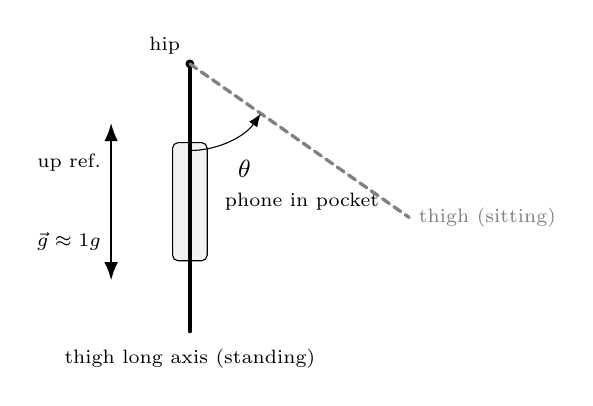
\begin{tikzpicture}[>=Latex, line cap=round, font=\small]
  \coordinate (hip) at (0,0);
  \coordinate (knee) at (0,-3.4);                         % standing thigh: straight down

  % phone, aligned to the standing thigh
  \draw[fill=black!5, rounded corners=2pt] (-0.22,-2.5) rectangle (0.22,-1.0);
  \node[anchor=west, font=\scriptsize] at (0.32,-1.75) {phone in pocket};

  % standing thigh long-axis
  \draw[very thick] (hip) -- (knee);
  \node[anchor=north, font=\scriptsize] at (0,-3.5) {thigh long axis (standing)};
  \fill (hip) circle (1.6pt);
  \node[anchor=south east, font=\scriptsize] at (hip) {hip};

  % gravity (down) and the calibrated up reference (up)
  \draw[->, thick] (-1.0,-1.75) -- (-1.0,-2.75)
        node[midway, left, font=\scriptsize] {$\vec{g}\approx 1g$};
  \draw[->, thick] (-1.0,-1.75) -- (-1.0,-0.75)
        node[midway, left, font=\scriptsize] {up ref.};

  % tilted thigh (sitting): straight-down rotated toward +x by 55 deg
  \coordinate (kneeT) at ({3.4*sin(55)},{-3.4*cos(55)});
  \draw[very thick, gray, densely dashed] (hip) -- (kneeT);
  \node[gray, anchor=west, font=\scriptsize] at (kneeT) {thigh (sitting)};

  % tilt arc between standing-down (270 deg) and tilted thigh (270+55 deg)
  \draw[->] (270:1.1) arc (270:325:1.1);
  \node[font=\small] at ({1.5*cos(297.5)},{1.5*sin(297.5)}) {$\theta$};
\end{tikzpicture}
\caption{Phone-in-pocket geometry. Standing, gravity runs $\sim 1g$ down the thigh long
axis and the calibrated ``up'' reference is its opposite. The run-time tilt $\theta$ is
the angle between the current mean gravity vector and this standing reference; it grows
as the thigh flexes (dashed, sitting).}
\label{fig:pocket}
\end{figure}

\paragraph{Magnetic baseline geometry.}
The same standing capture also fixes the locomotion baseline. From the captured window
the magnetometer yields two numbers: the field magnitude $|\vec B_0|$ and the
inclination $\iota_0$, the field's dip below horizontal measured against the
gravity-derived ``down'' (Figure~\ref{fig:mag}). \axis{locomotion\_state} stores these as
the baseline and, at run time, reads \textsf{in\_vehicle} when the live field has drifted
past a threshold from the baseline in either magnitude or inclination --- the steel mass
and motor of a vehicle distort the local field. The inclination is computed gravity-only
(no device quaternion), so the field's horizontal bearing (declination) is not recovered;
this is an honest limitation carried from the axis.

\begin{figure}[ht]
\centering
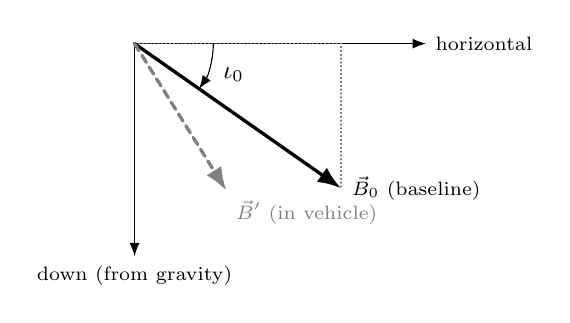
\begin{tikzpicture}[>=Latex, line cap=round, font=\small]
  \coordinate (O) at (0,0);
  % reference axes
  \draw[->] (O) -- (3.7,0) node[right, font=\scriptsize] {horizontal};
  \draw[->] (O) -- (0,-2.7) node[below, font=\scriptsize] {down (from gravity)};
  % baseline field B0 at inclination 35 deg below horizontal
  \coordinate (B) at ({3.2*cos(35)},{-3.2*sin(35)});
  \draw[->, very thick] (O) -- (B) node[right, font=\scriptsize] {$\vec B_0$ (baseline)};
  % right-triangle components (faint): horizontal and vertical parts of B0
  \draw[densely dotted, black!55] (O) -- ({3.2*cos(35)},0) -- (B);
  % inclination arc between horizontal and B0
  \draw[->] (1.0,0) arc (0:-35:1.0);
  \node at ({1.32*cos(-17.5)},{1.32*sin(-17.5)}) {$\iota_0$};
  % distorted field inside a vehicle (shorter, steeper)
  \coordinate (Bv) at ({2.2*cos(58)},{-2.2*sin(58)});
  \draw[->, very thick, gray, densely dashed] (O) -- (Bv);
  \node[gray, font=\scriptsize, anchor=north west] at (Bv) {$\vec B'$ (in vehicle)};
\end{tikzpicture}
\caption{Magnetic baseline geometry. At calibration the standing window fixes the field
magnitude $|\vec B_0|$ and the inclination $\iota_0$ (its dip below horizontal, against
the gravity-derived ``down''). At run time \axis{locomotion\_state} reads
\textsf{in\_vehicle} when the live field $\vec B'$ deviates past a threshold from this
baseline in magnitude or inclination; a vehicle's steel and motor distort the field.
Inclination is gravity-only, so declination (the horizontal bearing) is not recovered.}
\label{fig:mag}
\end{figure}

% ============================================================================
\section{The Five Axes}
% ============================================================================

Each axis is summarized below: what it infers, the physical idea, the single key
feature it turns on, and a pointer to its notebook. The notebooks are authoritative for
the full mathematics, derivation, and validation, including reported metrics, which are
deliberately not restated here. Across the axes, the rules were derived and frozen on
public smartphone and wearable activity datasets --- principally MotionSense
\citep{malekzadeh2019motionsense}, HHAR \citep{stisen2015hhar}, and PAMAP2
\citep{reiss2012pamap2} --- with UCI-HAR \citep{anguita2013ucihar} serving as the
project's baseline reference. Each axis's specific dataset is named in its notebook.

% ---------------------------------------------------------------------------
\subsection{activity\_state}
% ---------------------------------------------------------------------------
Infers how hard the body is working: sedentary, walking, running, or cycling. The
physical idea is that locomotor effort shows up as the energy and cadence of body
acceleration, and that magnitude features are orientation-invariant --- they do not
depend on how the phone sits in the pocket. The deciding features are the mean and
standard deviation of the body-acceleration magnitude (in $g$) and the cadence from its
autocorrelation; an energy split with a cadence tiebreaker resolves the walk/run
overlap band, and the gyroscope is used only to separate cycling in the low-motion
region. The axis reports a calibrated confidence with a reported ECE. See
\nb{maths/experiments/activity\_state.ipynb} for the full method and validation.

% ---------------------------------------------------------------------------
\subsection{movement\_regularity}
% ---------------------------------------------------------------------------
Infers how smooth and repeating the motion is, as a continuous score in $[0,1]$ (higher
is more regular). The physical idea is that regular gait makes the acceleration signal
self-similar one stride later, so a short-time autocorrelation of the acceleration
magnitude at the dominant lag measures regularity directly, following the trunk-
accelerometry method of \citet{moenilssen2004gait}.
The key quantity is the unbiased autocorrelation coefficient at the dominant period.
Confidence is deterministic; there is no ECE because the score has no categorical
ground-truth label to calibrate against --- which is correct for a continuous score, not
a gap. See \nb{maths/experiments/movement\_regularity.ipynb} for the full method.

% ---------------------------------------------------------------------------
\subsection{postural\_state}
% ---------------------------------------------------------------------------
Infers posture relative to the body: standing, sitting, in\_motion, lying, or
device\_resting. The physical idea is a thigh-tilt model: with the phone in the pocket,
the angle of gravity relative to the calibrated standing reference reports thigh
orientation. The key feature is the tilt $\theta$, the angle between the current mean
gravity vector and the calibrated standing ``up'' (Figure~\ref{fig:pocket}); standing
and sitting are separable by this angle on thigh/pocket placement. The flat-orientation
branch that distinguishes lying from device\_resting is untested on real data and is
flagged low-confidence in the reading rather than asserted. See
\nb{maths/experiments/postural\_state.ipynb} for the full model.

% ---------------------------------------------------------------------------
\subsection{locomotion\_state}
% ---------------------------------------------------------------------------
Infers whether the wearer is moving through space: stationary, on\_foot, or in\_vehicle.
The physical idea is two-stage. Stage~1 detects on-foot travel from gait rhythm via the
autocorrelation peak of body-acceleration magnitude. Stage~2, reached only when motion
is low or non-rhythmic, separates stationary from in\_vehicle by how far the magnetic
field has drifted from its self-calibrated startup baseline (field magnitude and
inclination), since a vehicle's mass of steel and its motor distort the local field. The
key feature is the baseline deviation of the field. This branch is a single-car
demonstration on PAMAP2, not a validation: proper evaluation needs a transportation-mode
dataset such as SHL \citep{gjoreski2018shl}, and the magnetometer baseline is sensitive
to device hard-iron bias and on-body magnets. A GPS-free direction for future work is to
fuse multiple vehicle cues --- the $\sim$4--15~Hz engine/road vibration band, spectral
aperiodicity, and accel/brake and cornering events \citep{hemminki2013transportation}
--- so that detection degrades gracefully and stays consistent with the privacy-first
principle.
See \nb{maths/locomotion\_state.ipynb} and \nb{maths/experiments/locomotion\_improved.ipynb}
for the full method.

% ---------------------------------------------------------------------------
\subsection{overall\_state}
% ---------------------------------------------------------------------------
Combines the four axes into a single reading: a situation label, an exertion level, and
a heart-rate context note. The physical idea is that the four kinematic facts together
pin down the situation more reliably than any one alone, and that a per-activity load
lookup maps the situation to an expected exertion.

The combination is a small fixed pipeline (Figure~\ref{fig:overall}). The situation is
the \emph{first} rule that matches in a fixed priority order; the exertion is a
per-activity load lookup, forced to zero in a vehicle; and the heart-rate note follows
from the exertion together with the regularity cue. The reported confidence --- the
``score'' --- is not an average: it is the \emph{minimum} confidence among only the axes
that actually drive the chosen situation, so a combined read is only as strong as its
weakest contributing ingredient.

\begin{figure}[ht]
\centering
\resizebox{\textwidth}{!}{%
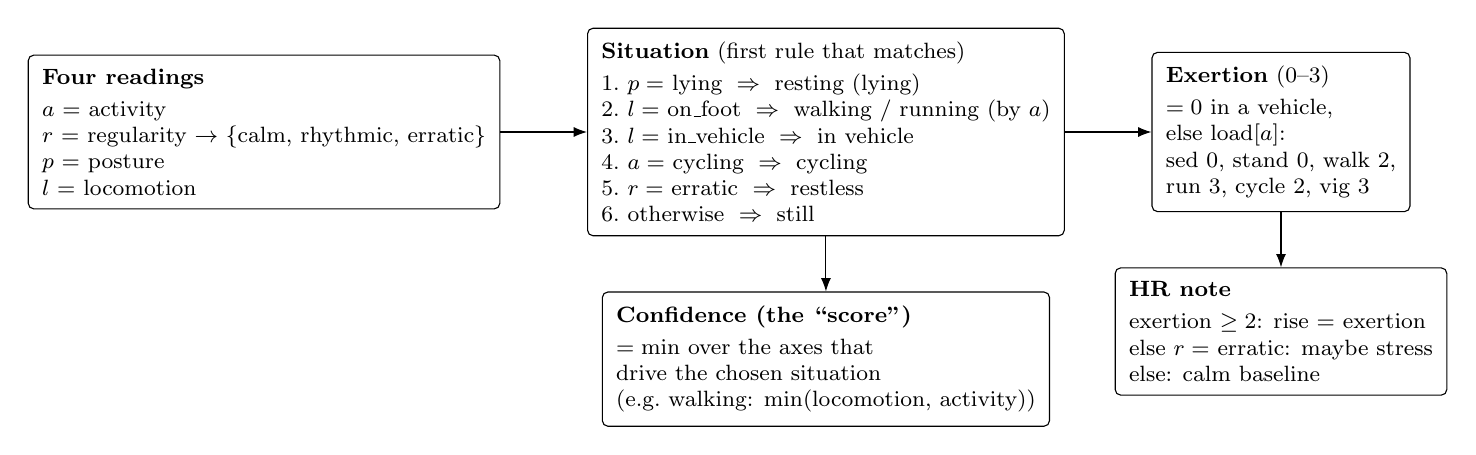
\begin{tikzpicture}[
  >=Latex, font=\footnotesize, node distance=7mm and 11mm,
  box/.style={draw, rounded corners=2pt, align=left, inner sep=5pt},
]
  \node[box] (in) {\textbf{Four readings}\\[2pt]
    $a$ = activity\\
    $r$ = regularity $\to$ \{calm, rhythmic, erratic\}\\
    $p$ = posture\\
    $l$ = locomotion};

  \node[box, right=of in] (sit) {\textbf{Situation} (first rule that matches)\\[2pt]
    1.\ $p =$ lying $\;\Rightarrow\;$ resting (lying)\\
    2.\ $l =$ on\_foot $\;\Rightarrow\;$ walking / running (by $a$)\\
    3.\ $l =$ in\_vehicle $\;\Rightarrow\;$ in vehicle\\
    4.\ $a =$ cycling $\;\Rightarrow\;$ cycling\\
    5.\ $r =$ erratic $\;\Rightarrow\;$ restless\\
    6.\ otherwise $\;\Rightarrow\;$ still};

  \node[box, right=of sit] (ex) {\textbf{Exertion} (0--3)\\[2pt]
    $=0$ in a vehicle,\\ else $\mathrm{load}[a]$:\\
    sed 0,\ stand 0,\ walk 2,\\ run 3,\ cycle 2,\ vig 3};

  \node[box, below=of ex] (note) {\textbf{HR note}\\[2pt]
    exertion $\ge 2$: rise $=$ exertion\\
    else $r =$ erratic: maybe stress\\
    else: calm baseline};

  \node[box, below=of sit] (conf) {\textbf{Confidence (the ``score'')}\\[2pt]
    $=\min$ over the axes that\\ drive the chosen situation\\
    (e.g.\ walking: $\min$(locomotion, activity))};

  \draw[->] (in)  -- (sit);
  \draw[->] (sit) -- (ex);
  \draw[->] (ex)  -- (note);
  \draw[->] (sit) -- (conf);
\end{tikzpicture}%
}
\caption{How \axis{overall\_state} combines the four readings. The situation is the first
matching rule in a fixed priority order; the exertion is a per-activity load lookup
(zeroed in a vehicle); the heart-rate note follows from the exertion and the regularity
cue. The headline confidence is the minimum confidence among only the axes that drive the
chosen situation.}
\label{fig:overall}
\end{figure}

\paragraph{Worked example.}
Take $a =$ walking, regularity score $0.72$ (so $r =$ rhythmic), $p =$ standing, and
$l =$ on\_foot. Rule~1 does not fire ($p \neq$ lying); rule~2 does ($l =$ on\_foot, and
$a \neq$ running), giving the situation \textsf{walking}. The wearer is not in a vehicle,
so the exertion is $\mathrm{load}[\text{walking}] = 2$; because exertion $\ge 2$, the note
is ``HR rise $=$ physical exertion (expected)''. Walking is driven by the locomotion and
activity axes, so the confidence is the smaller of those two percentages: with
illustrative per-axis values of $78\%$ (locomotion) and $84\%$ (activity), the headline
confidence is $78\%$, limited by locomotion. The combined reading is therefore
\{situation: walking, exertion: 2, note: HR rise expected, confidence: 78\%\}. See
\nb{maths/overall\_state.ipynb} for the full combiner.

% ============================================================================
\section{Convergence}
% ============================================================================

The five axes were frozen separately, on different datasets and body placements, and
then run together off one pocket stream. Bringing them onto a single stream is itself a
test: an axis tuned on one placement or unit convention fails visibly when fed the
shared pocket window, and the convergence work surfaced and fixed several such real
bugs. These included unit mismatches (thresholds carried in $\mathrm{m/s^2}$ applied to
features expressed in $g$, off by a factor of $\sim 9.81$), a thigh-tilt inversion in
which a flat reference made a flat phone read as standing, and magnetometer baselines
that had to become self-calibrated at startup rather than assumed. Each fix is recorded
where it was made; the convergence procedure is documented in
\nb{maths/experiments/convergence\_test.ipynb}.

% ============================================================================
\section{Limitations and Future Work}
% ============================================================================

The honest limitations of the current system are consolidated here.

\begin{itemize}
  \item \textbf{Placement and labeled calibration are dataset luxuries.} Several axes
        were derived on chest-worn or labeled data, whereas deployment is pocket-worn
        and unlabeled. A chest signal is not a pocket signal, and a deployed device has
        no labels to calibrate against; the system therefore relies on the startup
        self-calibration of Section~\ref{sec:calibration} to recover the references it
        cannot assume.
  \item \textbf{Locomotion is a single-car demonstration.} The stationary-versus-vehicle
        branch has been shown on one car in PAMAP2, not validated. Proper evaluation
        needs a transportation-mode dataset such as SHL \citep{gjoreski2018shl}, and the
        magnetometer baseline remains sensitive to device hard-iron bias and on-body
        magnets.
  \item \textbf{The lying branch is untested.} The flat-orientation distinction between
        lying and device\_resting has no real-data validation and is reported
        low-confidence rather than asserted.
  \item \textbf{Transition windows are untested.} A 5~s window that straddles a change
        of activity mixes two states; behaviour across such transitions has not been
        characterized.
  \item \textbf{Thresholds are provisional.} A number of thresholds were carried from
        the placement or dataset they were tuned on and are marked provisional in the
        configuration; they need re-tuning on deployment data.
  \item \textbf{GPS-free multi-cue locomotion.} The most promising direction is the
        fused vehicle-cue detector described above
        \citep{hemminki2013transportation}, which would improve locomotion robustness
        without adding any location tracking.
\end{itemize}

% ============================================================================
\bibliographystyle{plainnat}
\bibliography{references}
% ============================================================================

\end{document}
